\documentclass[a4paper, 12pt]{report}
\usepackage[french]{babel}
\usepackage[utf8]{inputenc}
\usepackage[T1]{fontenc}
\usepackage{graphicx}
\usepackage{geometry}
\usepackage{tabularx}
\usepackage{caption}
%\usepackage[usenames,dvipsnames,svgnames,table]{xcolor}
%\usepackage{pdfpages}
%\geometry{hmargin=2.5cm,vmargin=2.5cm}

% Title Page
\begin{document}
\begin{titlepage}
\newcommand{\HRule}{\rule{\linewidth}{0.5mm}}

\begin{center}

\HRule \\[0.4cm]
{ \huge Projet : Exécution symbolique et tests structurels}\\[0.4cm]
\HRule \\[2cm]

\vspace{2cm}

Ayaz Badouraly \& Venceslas Danguy des Déserts

\vspace{2cm}

Enseignante :
Mme Pascale Le Gall


\end{center}
\end{titlepage}

%\maketitle
%\newpage


\tableofcontents
\newpage

\chapter{Architecture du projet}

\section{Pipe de traitement}

Le code se divise en trois grandes parties : parsing du programme dans le langage WHILE, vérification de critères sur ce programme, génération des tests pour les critères.

\subsection{Parsing}

Le parsing consiste, à partir d'un programme écrit en langage WHILE, à obtenir un graphe de contrôle (CFG) représentant le dit programme. On passe pour cela par une étape intermédiaire : un arbre de syntaxe abstraite, ou AST. L'AST est une représentation du code du programme sous forme d'arbre, tandis que le CFG représente vraiment le flux du programme. 

%Insérer exemples AST et CFG associés

\subsubsection{Génération de l'AST}

Nous utilisons pour ce faire la librairie Python ply, qui fournit une implémentation en Python du duo lex/yacc. Lex tokenize le programme en entrée en fonction de la grammaire définie, tandis que yacc prend l'entrée tokenizée et fournit l'AST. Nous utilisons la librairie \textit{anytree} pour manipuler les arbres.

\subsubsection{Conversion de l'AST au CFG}

Il faut ensuite traduire cet AST en CFG. On utilise pour cela un algorithme récursif qui va parcourir l'arbre et construire le CFG. Chaque exécution de la fonction récursive renvoie un morceau de graphe ainsi que des arêtes sortantes à relier.

Ainsi, la conversion d'un arbre ne contenant en tout et pour tout qu'une assignation va renvoyer un noeud labellisé et une arête sortante de ce noeud portant une condition \textit{True} et une commande \textit{Assign}.

La conversion d'un arbre contenant un noeud While va relier les arêtes sortantes du graphe du sous-arbre au noeud parent de façon à former une boucle, etc.

On ajoute enfin un tag sur les noeuds correspondant à des instructions \textit{If} ou \textit{While} pour faciliter la vérification et la génération des tests.

Les graphes sont gérés par la librairie python \textit{networkx}.

\subsection{Vérification de critères}

Nous sommes donc désormais capables d'obtenir le CFG associé à un programme écrit en langage WHILE. Nous voulons maintenant \textit{vérifier} des critères de tests pour ce programme, c'est à dire, étant donné un jeu de tests (données de départs), dire si les tests couvrent un ensemble de cas (chemins d'exécution) précis.

Il faut donc commencer par exécuter le programme avec le jeu de test. Ceci se fait assez facilement, il suffit de parcourir le graphe de contrôle en maintenant un état (ensemble des variables et de leurs valeurs) et en choisissant, à chaque branchement, l'arête dont la condition est vérifiée par l'état.

On obtient ainsi un ensemble de chemins d'exécution (un par valuation de départ).

Parallèlement, on a un critère de test, c'est à dire un ensemble de chemins par lesquels nous voulons passer. Ainsi le critère \textit{Toutes les affectations} demande-t-il qu'à la fin de l'exécution de tous les tests, on soit passé au moins une fois par chaque arête portant une commande \textit{Assign}.

Chaque critère possède son propre algorithme de génération d'éléments à vérifier en fonction du programme (bien que l'on puisse toujours se ramener à un ensemble de chemins, il était parfois plus simple de considérer un ensemble de noeuds ou d'arêtes par lesquels il faut passer).

Il suffit ensuite de faire l'intersection des deux ensembles \textit{\{Chemins exécutés lors de la phase du test\}} et \textit{\{Chemins à vérifier imposés par le critère\}}.


\section{Choix de conception}

\section{Limitations adoptées}

\section{Organisation du code}

Le code est organisé en modules.

\begin{description}
\item[- astree :] Contient notre structure d'AST avec les commandes et opérations définies par la sémantique opérationnelle de WHILE.
\item[- cfgraph :] Code utilisé pour exécuter un test sur le programme. Le module utils, en particulier, contient toutes les fonctions du graphe nécessaires pour générer les éléments à vérifier pour chaque critère.
\item[- syntax :] Contient le code du lexeur et du parseur ainsi que leur configuration
\item[- tests :] Ce dossier contient le coeur du projet. Le module \textit{tester} contient la logique de vérification des critères : récupération des éléments à vérifier, analyse des chemins d'exécutions des tests pour y trouver les éléments. Le module \textit{generator} gère la génération des jeux de tests en faisant appel au solveur \textit{Z3}.
\item[- utils :] Contient notamment la conversion de l'AST vers le CFG.
\item[- input :] Contient des exemples de programmes sur lesquels on peut vérifier les critères.
\item[- output :] Exemples de graphes (images). 
\end{description}

\chapter{Vérification des critères et génération des tests}
% D'après le sujet, pour chaque critère :
% - Jeux de tests satisfaisant et ne satisfaisant pas le critère
% - Mécanisme de vérification
% - Mécanisme de génération
% Et en général : relations d'ordre entre les critères

\section{Toutes les affectations}
\label{sec:affectations}
On va travailler sur le programme suivant :

\begin{minipage}{0.46\textwidth}
\begin{verbatim}
1:  if (x <= 0) {
2:      x := -x;
    } else {
3:      x := 1 - x;
    }

4:  if (x == 1) {
5:      x := 1;
    } else {
6:      x := x + 1;
    }
\end{verbatim}
\end{minipage}
\begin{minipage}{0.46\textwidth}
	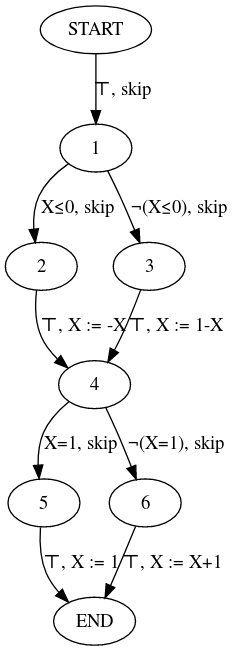
\includegraphics[scale=0.5]{pics/simpleCFG.png}
	\captionof{figure}{CFG associé}
\end{minipage}

%Ajouter AST + CFG en illustration de la partie précédente

Le critère \textit{Toutes les affectations} demande à ce que tous les labels d'affectations (ici : $2, 3, 5, 6$) apparaissent au moins une fois dans l'un des chemins d'exécution correspondant aux données de tests.

Si on prend pour jeu de test :

\[ \{
	\{ X : -1\},
	\{ X : 1\}
\} \]

On obtient les chemins d'exécutions suivants :
\begin{description}
\item[$\{ X : -1\}$ : ] $1, 2, 4, 5$
\item[$\{ X : 1\}$ : ] $1, 3, 4, 6$
\end{description}

On est donc passé au moins une fois par chaque label associé à une affectation : le critère est vérifié sur ce programme et ce jeu de test.

Si, en revanche, on s'était contenté d'un unique test $\{ X : -1\}$, on ne serait pas passé par les noeuds $3$ et $6$, et le critère n'aurait pas été vérifié.

Dans la pratique, étant donné un CFG, on récupère l'ensemble des noeuds (labels) tels qu'une arête sortante de ce noeud porte une affectation. Ceci se fait très facilement en parcourant l'ensemble des arêtes (sans notion de chemin ici).
Il suffit ensuite de regarder lesquels de ces noeuds sont (ou non) dans les chemins des tests.

\section{Toutes les décisions}

On travaille toujours sur le programme défini en \ref{sec:affectations}.

Le critère \textit{Toutes les décisions} demande à ce que l'on passe au moins une fois par toutes les arêtes associées à une expression booléenne. Il s'agit, en bref, de toutes les arêtes sortantes des noeuds \textit{if} et \textit{while}, ce qui est équivalent à dire qu'il faut passer par les noeuds de destination de ces arêtes.

Ici, il faut donc passer par les noeuds $2, 3, 5, 6$. On retombe dans ce cas très simple sur les même éléments que le critère \textit{Toutes les affectations}, et le même jeu de tests vérifie donc les deux critères.
\section{Tous les \textit{k}-chemins}
\section{Toutes les \textit{i}-boucles}
\section{Toutes les définitions}
\section{Toutes les utilisations}
\section{Tous les DU-chemins}
\section{Toutes les conditions}
\end{document}